\documentclass[review]{elsarticle}

\usepackage[colorlinks]{hyperref}
\usepackage[colorinlistoftodos]{todonotes}
\usepackage{verbatim}
\usepackage[utf8]{inputenc}
\usepackage[T1]{fontenc}
\usepackage{adjustbox}
\usepackage{multirow}
\usepackage{longtable}
\usepackage{booktabs}
\usepackage{lineno,hyperref}
\usepackage{listings}
\modulolinenumbers[5]

\journal{colleagues for review}

%%%%%%%%%%%%%%%%%%%%%%%
%% Elsevier bibliography styles
%%%%%%%%%%%%%%%%%%%%%%%
%% To change the style, put a % in front of the second line of the current style and
%% remove the % from the second line of the style you would like to use.
%%%%%%%%%%%%%%%%%%%%%%%

%% Numbered
%\bibliographystyle{model1-num-names}

%% Numbered without titles
%\bibliographystyle{model1a-num-names}

%% Harvard 
%\bibliographystyle{model2-names.bst}\biboptions{authoryear}

%% Vancouver numbered
%\usepackage{numcompress}\bibliographystyle{model3-num-names}

%% Vancouver name/year
%\usepackage{numcompress}\bibliographystyle{model4-names}\biboptions{authoryear}

%% APA style
\bibliographystyle{model5-names}\biboptions{authoryear}

%% AMA style
%\usepackage{numcompress}\bibliographystyle{model6-num-names}

%% `Elsevier LaTeX' style
%\bibliographystyle{elsarticle-num}
%%%%%%%%%%%%%%%%%%%%%%%

\begin{document}

\begin{frontmatter}

%% Title, authors and addresses

\title{Shape difference or shape change? Inter-regional variation in Gahagan biface morphology}

%% use the tnoteref command within \title for footnotes;
%% use the tnotetext command for the associated footnote;
%% use the fnref command within \author or \address for footnotes;
%% use the fntext command for the associated footnote;
%% use the corref command within \author for corresponding author footnotes;
%% use the cortext command for the associated footnote;
%% use the ead command for the email address,
%% and the form \ead[url] for the home page:
%%
%% \title{Title\tnoteref{label1}}
%% \tnotetext[label1]{}
%% \author{Name\corref{cor1}\fnref{label2}}
%% \ead{email address}
%% \ead[url]{home page}
%% \fntext[label2]{}
%% \cortext[cor1]{}
%% \address{Address\fnref{label3}}
%% \fntext[label3]{}


%% use optional labels to link authors explicitly to addresses:
%% \author[label1,label2]{<author name>}
%% \address[label1]{<address>}
%% \address[label2]{<address>}
%% Group authors per affiliation:
\author{Robert Z. Selden, Jr.\textsuperscript{a,b,c*} and John E. Dockall\textsuperscript{d,e}}
\address[1]{Heritage Research Center, Stephen F. Austin State University, United States}
\address[2]{Cultural Heritage Department, Jean Monnet University, France}
\address[3]{ORCID ID \href{http://orcid.org/0000-0002-1789-8449}{0000-0002-1789-8449}}
\address[4]{Prewitt and Associates, Inc., United States}
\address[5]{ORCID ID \href{http://orcid.org/0000-0002-0940-7144}{0000-0002-0940-7144}}
\cortext[cor1]{Corresponding author, Robert Z. Selden, Jr. (zselden@sfasu.edu)}

\begin{abstract}
This investigation aggregates intact or reconstructed Gahagan bifaces from Caddo and central Texas sites to test the hypothesis that Gahagan biface morphology differs between the two regions. The bifaces were scanned, then analysed using the tools of geometric morphometrics. Results provide a preview of the morphological differences that occur in Gahagan bifaces found at Caddo and central Texas sites. The size disparity represents an inversion of theoretical constructs that posit a decrease in tool size thought to articulate with an increase in distance from raw material source, as the bulk of the Caddo sample is thought to have been produced of Edwards chert from central Texas. One hypothesis (shape difference) posits that the contrasting morphologies may represent two discrete communities of practice; one (central Texas) that potentially utilised the bifaces for more practical purposes, and the other (Caddo) that enlisted Gahagan bifaces in burial and ritualistic activities. An alternative hypothesis (shape change) posits that Gahagan bifaces may have served multiple functions in Caddo society that differ in their deployment within and beyond the southern Caddo area.
\end{abstract}

\begin{keyword}
bifaces \sep NAGPRA \sep 3D \sep geometric morphometrics \sep museum studies
\end{keyword}

\end{frontmatter}

\linenumbers

\section*{}

\begin{quote}
The mathematical definition of a ``form'' has a quality of precision which was quite lacking in our earlier stage of mere description; it is expressed in few words, or in still briefer symbols, and these words or symbols are so pregnant with meaning that thought itself is economised \citep[720-721]{RN11532}.    
\end{quote}

This contribution follows a recent study of Gahagan biface morphology that enlisted the three largest samples from the Gahagan Mound (16RR1), George C. Davis (41CE19), and Mounds Plantation (16CD12) sites in the southern Caddo area (Figure 1) \citep{RN11783}. The results of that study indicated a significant difference in shape for Gahagan bifaces found at Mounds Plantation site when compared with those found at the Gahagan Mound and George C. Davis sites \citep[Figure 7]{RN11783}. The test for morphological disparity indicated that the sample from Gahagan Mound occupied a significantly greater range of morphospace than the sample from Mounds Plantation, providing limited evidence for discussions of specialisation and diversity. Morphological integration was also significant, meaning those traits used to characterise Gahagan biface shape (blade and base) were found to vary in a coordinated manner. The results confirmed the supposition advanced by \cite{RN3684} that the assemblage of Gahagan bifaces from the George C. Davis site compares favourably with those reported from the Gahagan Mound site \citep{RN5274,RN2740}.

The Gahagan type was suggested by Clarence H. Webb at the Caddo Conference in 1970 \citep{RN3684}, and was intended as a replacement for what \cite{RN800} had previously called Copena knives based upon similarities in form, but not technology \citep{RN3684}, between specimens found at the George C. Davis site and those reported by \cite{RN11562} in Alabama. Gahagan bifaces are currently thought to differ from Copena bifaces in morphology and technology, and were named for the finely-crafted bifaces found by \cite{RN2740} at Gahagan Mound \citep{RN3684}. \citet[22]{RN4924} later advanced a useful technological and morphological description for the type. Like the Gahagan bifaces from the George C. Davis site, those from the Gahagan Mound and Mounds Plantation sites demonstrate a relatively high degree of intra-type morphological variation. The addition of new specimens from known Caddo sites (Doc Marks and Pelican) are contrasted with those found at central Texas sites (Bastrop State Park and Doerge Collection), as well as an unprovenienced collection from the Brazos Valley Museum of Natural History (BVMNH) (Figure 2), provide those data needed to test whether Gahagan biface morphology in central Texas differs from those found at Caddo sites in east Texas. The Doerge collection is the largest collection of Gahagan bifaces to be found outside of the southern Caddo area \citep[Table 5]{RN4924}.

\begin{figure}[ht!]\centering
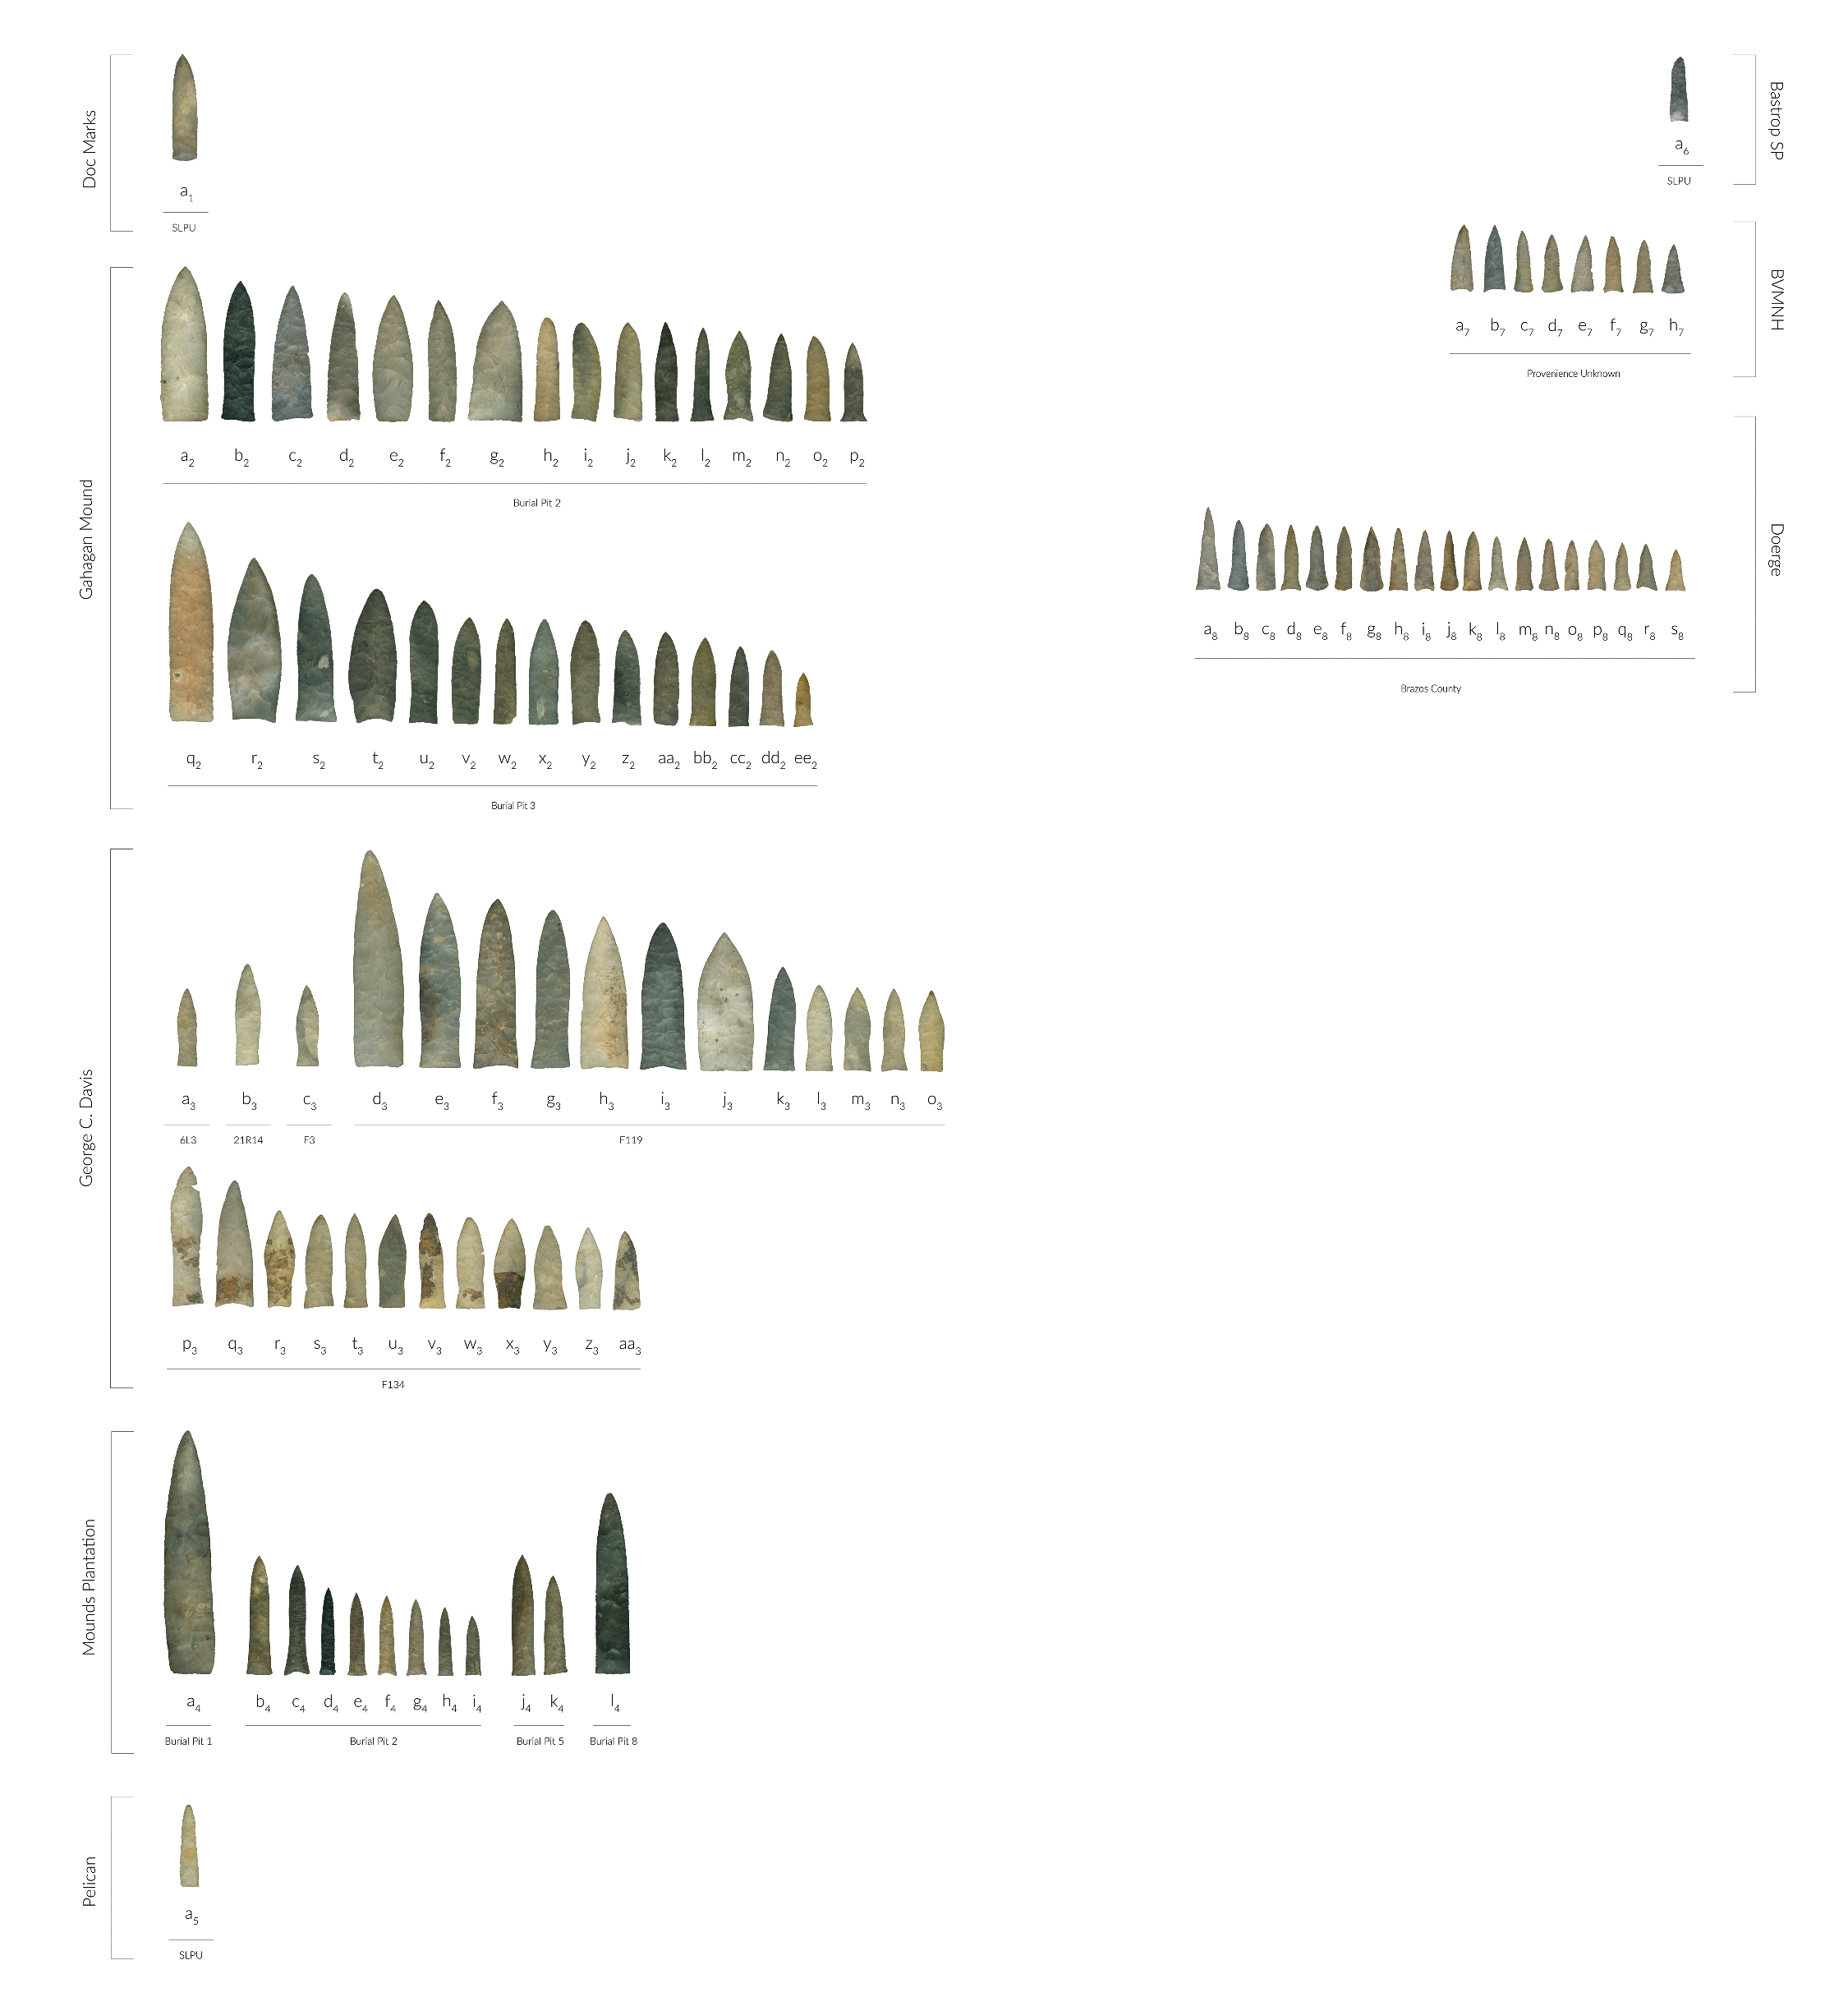
\includegraphics[width=\linewidth]{fig2}
\caption{Gahagan bifaces from known Caddo (left) and central Texas sites (right) organised by context and length; a1, Doc Marks; a2, 569; b2, 543; c2, 551; d2, 541; e2, 546; f2, 544; g2, 545; h2, 489; i2, 532; j2, 548; k2, 550; l2, 533; m2, 549; n2, 547; o2, 490; p2, 542; q2, 593; r2, 666; s2, 605; t2, 622; u2, 606; v2, 609; w2, 623; x2, 608; y2, 607; z2, 662; aa2, 611; bb2, 610; cc2, 612; dd2, 613; ee2, 614; a3, ET221-993; b3, ET221-1260A; c3, ET221-1016; d3, 463-1; e3, 424-39; f3, 424-53; g3, 424-50; h3, 424-41; i3, 424-221; j3, 424-218; k3, 463-16; l3, 424-230; m3, 463-23; n3, 424-169; o3, 424-33; p3, 4078-8; q3, 4078-9; r3, 4078-11; s3, 4078-72; t3, 4078-45; u3, 4078-12; v3, 4078-13; w3, 4078-72; x3, 4078-14; y3, 4078-32; z3, 4078-22; aa3, 4078-14; a4, 3Ba90; b4, 3Bb6; c4, 3Bb1; d4, ThnBlk; e4, 3Bb7; f4, 3Bb3; g4, 3Bb4; h4, 3Bb8; i4, 3Bb5; j4, Case2LG; k4, Case2SM; l4, LGGray. Bifaces w2, z2, and aa3 were not used in the analysis due to basal fractures, but are included here for visual comparative purposes.}
\label{fig:fig2}
\end{figure}

This effort represents the first formal comparison of Gahagan biface morphology across archaeological regions. Preliminary observations point to significant morphological differences between Gahagan bifaces recovered from Caddo and central Texas sites. Gahagan bifaces are a descriptive type that includes both morphological and chronological characteristics \citep{RN20847}, which has long been used as a diagnostic artefact type that articulates with Formative or Early Caddo occupations. Should the morphology of Gahagan bifaces from central Texas be found to differ from those recovered from the southern Caddo area, additional theoretical explanations may be warranted. One possibility (shape difference) may be that two communities of practice existed for Gahagan bifaces. An alternative explanation (shape change) may be situational, demonstrating that Gahagan bifaces served multiple functions within Caddo society. A third explanation is that both a shape difference and a shape change may be evidenced in Gahagan bifaces that may be further demarcated through an examination of context and seriation.

\subsection*{Context}

The flexuous blade shapes associated with Gahagan bifaces from Burial 1 at the Gahagan Mound site led to the initial interpretation that they were knives \citep[Figures 18-21]{RN2740}. A subsequent investigation at the Gahagan Mound site classified bifaces into two different biface types (neither of them Gahagan); one made of dull gray chert with a square base and a symmetrical or curved knife form, and the other made of semi-translucent flint with a curved base and more strongly curved sides \citep{RN5274}. In Burial Pit 2 at Gahagan Mound \citep[Plate 21]{RN5274}, one Gahagan biface (Figure ~\ref{fig:fig2}, a2) \citep[Plate 27, No. 1, 3]{RN5274} was found near the left shoulder of an adult male (Skeleton 3), but most artefacts were recovered near the northwest margin of the burial pit, including the remaining Gahagan bifaces associated with that context. In Burial Pit 3 at Gahagan Mound \citep[Plate 23, 1]{RN5274}, one Gahagan biface was found near the left femur of Skeleton 1 (Figure ~\ref{fig:fig2}, r2) \citep[Plate 27, No. 1, 2]{RN5274}. Similar to Burial Pit 2, most of the artefacts from Burial Pit 3 were found along the northwest margin, including the remainder of Gahagan bifaces from that context \citep{RN5274}.

At the George C. Davis site, two Gahagan bifaces were found outside of mound or feature contexts (Figure ~\ref{fig:fig2}, a3 and b3), and their feature assignments (6L3 and 21R14) articulate with the excavation grid used by \cite{RN800}. Feature 3 is associated with a 27-foot diameter ring of 35 postholes located east of Mound A \citep[Figure 4]{RN800}. One Gahagan biface (Figure ~\ref{fig:fig2}, c3) was found in the outlining postholes \cite{RN800}.

Feature 134 is associated with a Stage I burial feature at the George C. Davis site that predates the construction of Mound C, and contained eight individuals (Story 1997, 1972). One large (48 cm), well-thinned biface that Story (1997:22) listed as a “Gahagan?” biface was found near the right leg of Skeleton 5. Shafer (1973:Figure 19x) included this specimen—and one additional large specimen from Feature 119 (Shafer 1973:Figure 19w)—in his Group 2 bifaces due to a lack of the fine pressure-flaked margins definitive of Group 1 (Gahagan) bifaces (Shafer 1973). Nine Gahagan bifaces from Feature 134 were recovered from Concentration 2; seven (see Figure 2p2-r2, u2, v2, x2, and aa3) were found “about and under gray pigment,” and two others were found outside of the pigmented area (see Figure 2s2, w2) (Story 1997:21-23 and Figure 12). Organic residue can still be found on a selection of these Gahagan bifaces (Selden Jr., Dockall, and Shafer 2018a:Figure 2), which Shafer (1973:228) notes, “may be the remains of leather or bark sheaths or cane wrapping.” Three additional Gahagan bifaces (see Figure 2t2, y2, and z2) were found in Concentration 3 (Story 1997:21-22 and Figure 12).

Feature 119 (Story 1997:Figures 13-18) articulates with a Stage II burial feature at the George C. Davis site that can be traced from the surface of the second mound stage, and included offerings associated with two layers (Story 1997, 1969, 1972). The first layer offerings include Gahagan bifaces from Concentration 1 (see Figure 2o2), Concentration 2 (see Figure 2e2, g2, h2, and n2), and Concentration 3 (see Figure 2f2, i2, j2, and l2). Second layer offerings include Gahagan bifaces associated with Concentration 1 (see Figure 2d2), Concentration 3 (see Figure 2m2), and Skeleton 1 (see Figure 2k2). 

Burial Pit 2 at Mounds Plantation is the only context that contained a single individual, and Webb and McKinney (1975:97) noted that the Gahagan bifaces from Burial 2 exhibit “fine edge retouch [that] leaves the edges with almost no serration or irregularity, altogether the finest flint knapping that we have seen from a Caddoan site” (see Figure 2b3-i3). The bifaces from Burial Pit 2 at Mounds Plantation were found in a bundle, but those from Burial Pit 5 articulate with the males of Groups 1 and 2 (see Figure 2j3 and k3, respectively), and were found in a context parallel to the left forearm, pointed toward the hand (Webb and McKinney 1975:Figure 5). The biface from Burial Pit 8 at Mounds Plantation (see Figure 2l3) was found in the same position on the left forearm; however, the largest biface (Burial Pit 1, Skeleton 1; see Figure 2a3) was found across the chest of that individual (Webb and McKinney 1975).

McKinney posited that Gahagan bifaces may have been carried in a sheath attached to the left forearm (Webb and McKinney 1975). Similarly, Shafer (1973) noted that---at the George C. Davis site---edge modification was confined to traces of polish and smoothing along the widest blade segments and near the tip on burial specimens, was more pronounced on specimens from non-mound contexts, and possibly represented sheath wear. The polish that Shafer (1973) discussed supports McKinney’s hypothesis (Webb and McKinney 1975), where the tip and lateral edges of the biface became polished while being worn in a sheath on the left forearm with the tip pointed toward the hand.

DISCUSSION RE: LACK OF CONTEXT FOR CTX SPECIMENS...THUS FAR

\bibliography{mybibfile}

\end{document}